% This is samplepaper.tex, a sample chapter demonstrating the
% LLNCS macro package for Springer Computer Science proceedings;
% Version 2.20 of 2017/10/04
%
\documentclass[runningheads]{llncs}
%
\usepackage{amsmath}
\usepackage{graphicx}
\usepackage{subfigure}
\usepackage{float}
\usepackage{booktabs}

% Used for displaying a sample figure. If possible, figure files should
% be included in EPS format.
%
% If you use the hyperref package, please uncomment the following line
% to display URLs in blue roman font according to Springer's eBook style:
% \renewcommand\UrlFont{\color{blue}\rmfamily}

\begin{document}
%
\title{A CNN Based AMOLED Display Ageing Compensation Quality Evaluation System\\
ECE657A Spring2020 Project Report}
%
\titlerunning{AMOLED Display Ageing Compensation Quality Evaluation System}
% If the paper title is too long for the running head, you can set
% an abbreviated paper title here
%
\author{Alyssa Yiqin Huang\orcidID{20868286} \and
Tong Liu\orcidID{20809932}}
%

% First names are abbreviated in the running head.
% If there are more than two authors, 'et al.' is used.
%
\institute{Electrical and Computer Engineering, University of Waterloo\\
200 University Ave W, Waterloo, ON N2L 3G1, Ontario, Canada\\
\email{\{y672huan,t344liu\}@uwaterloo.ca}}
%
\maketitle              % typeset the header of the contribution
%
\begin{abstract}
An accurate and quick display luminance uniformity evaluation function plays a key feedback role for the automated AMOLED Display ageing compensation evaluation system. In this report we discuss a CNN  autoencoder based luminance uniformity evaluation system which we designed and implemented for AMOLED display ageing compensation performance evaluation. Within a short period of time we are able to classify an aged AMOLED display had a high quality compensation, or a low quality compensation. The result has relatively high accuracy, and the system could make classification decision for every sample image in about 1 second.

\keywords{ CNN autoencoder\and Active Matrix Organic Light-Emitting Diode\and AMOLED Display Aging\and AMOLED Display Aging Compensation.}
\end{abstract}
%
%
%
\section{Introduction}
The AMOLED display panel has been widely used as a high-end smartphone display, TV display and automotive car informatic display. A major long-term performance issue of AMOLED display is OLED material ageing, which is the luminance performance drop at the aged area cause nonuniformity issue on AMOLED display.  As Figure. \ref{fig:1} shows, the luminance nonuniformity shows a symptom is called burn-in.
To solve the OLED ageing issue and eliminate burn-in on AMOLED display, Ignis Innovation Inc. has developed a state of art OLED ageing compensation solution to solve the OLED ageing problem as Figure.  \ref{fig:2} shows.

However, traditional methods to evaluate the quality of OLED ageing compensation is processed based on human vision. It takes much time. Its evaluations vary from person to person and difficult to compare between evaluation results. Thus, evaluating the quality of OLED ageing compensation with a speedy and accurate approach is a technical challenge.

During the ECE657A project, we tried to develop an OLED ageing compensation evaluation function to solve the above technical challenge using the knowledge and techniques we have learned in this course. We build a prototype system which is having conceptual functionality works as expected. The system can classify the AMOLED display OLED ageing compensation quality is “good” or “bad”. Good compensation quality means with OLED ageing compensation, the brightness uniformity on the OLED display is beyond a certain threshold. Ideally, there will be no visible burn-in ageing area on display while the smartphone is running normally. Bad compensation quality means that with OLED ageing compensation, the brightness uniformity on the OLED display is below a certain threshold. There could be some visible burn-in area still showing on OLED display.

\begin{figure}
    \centering
    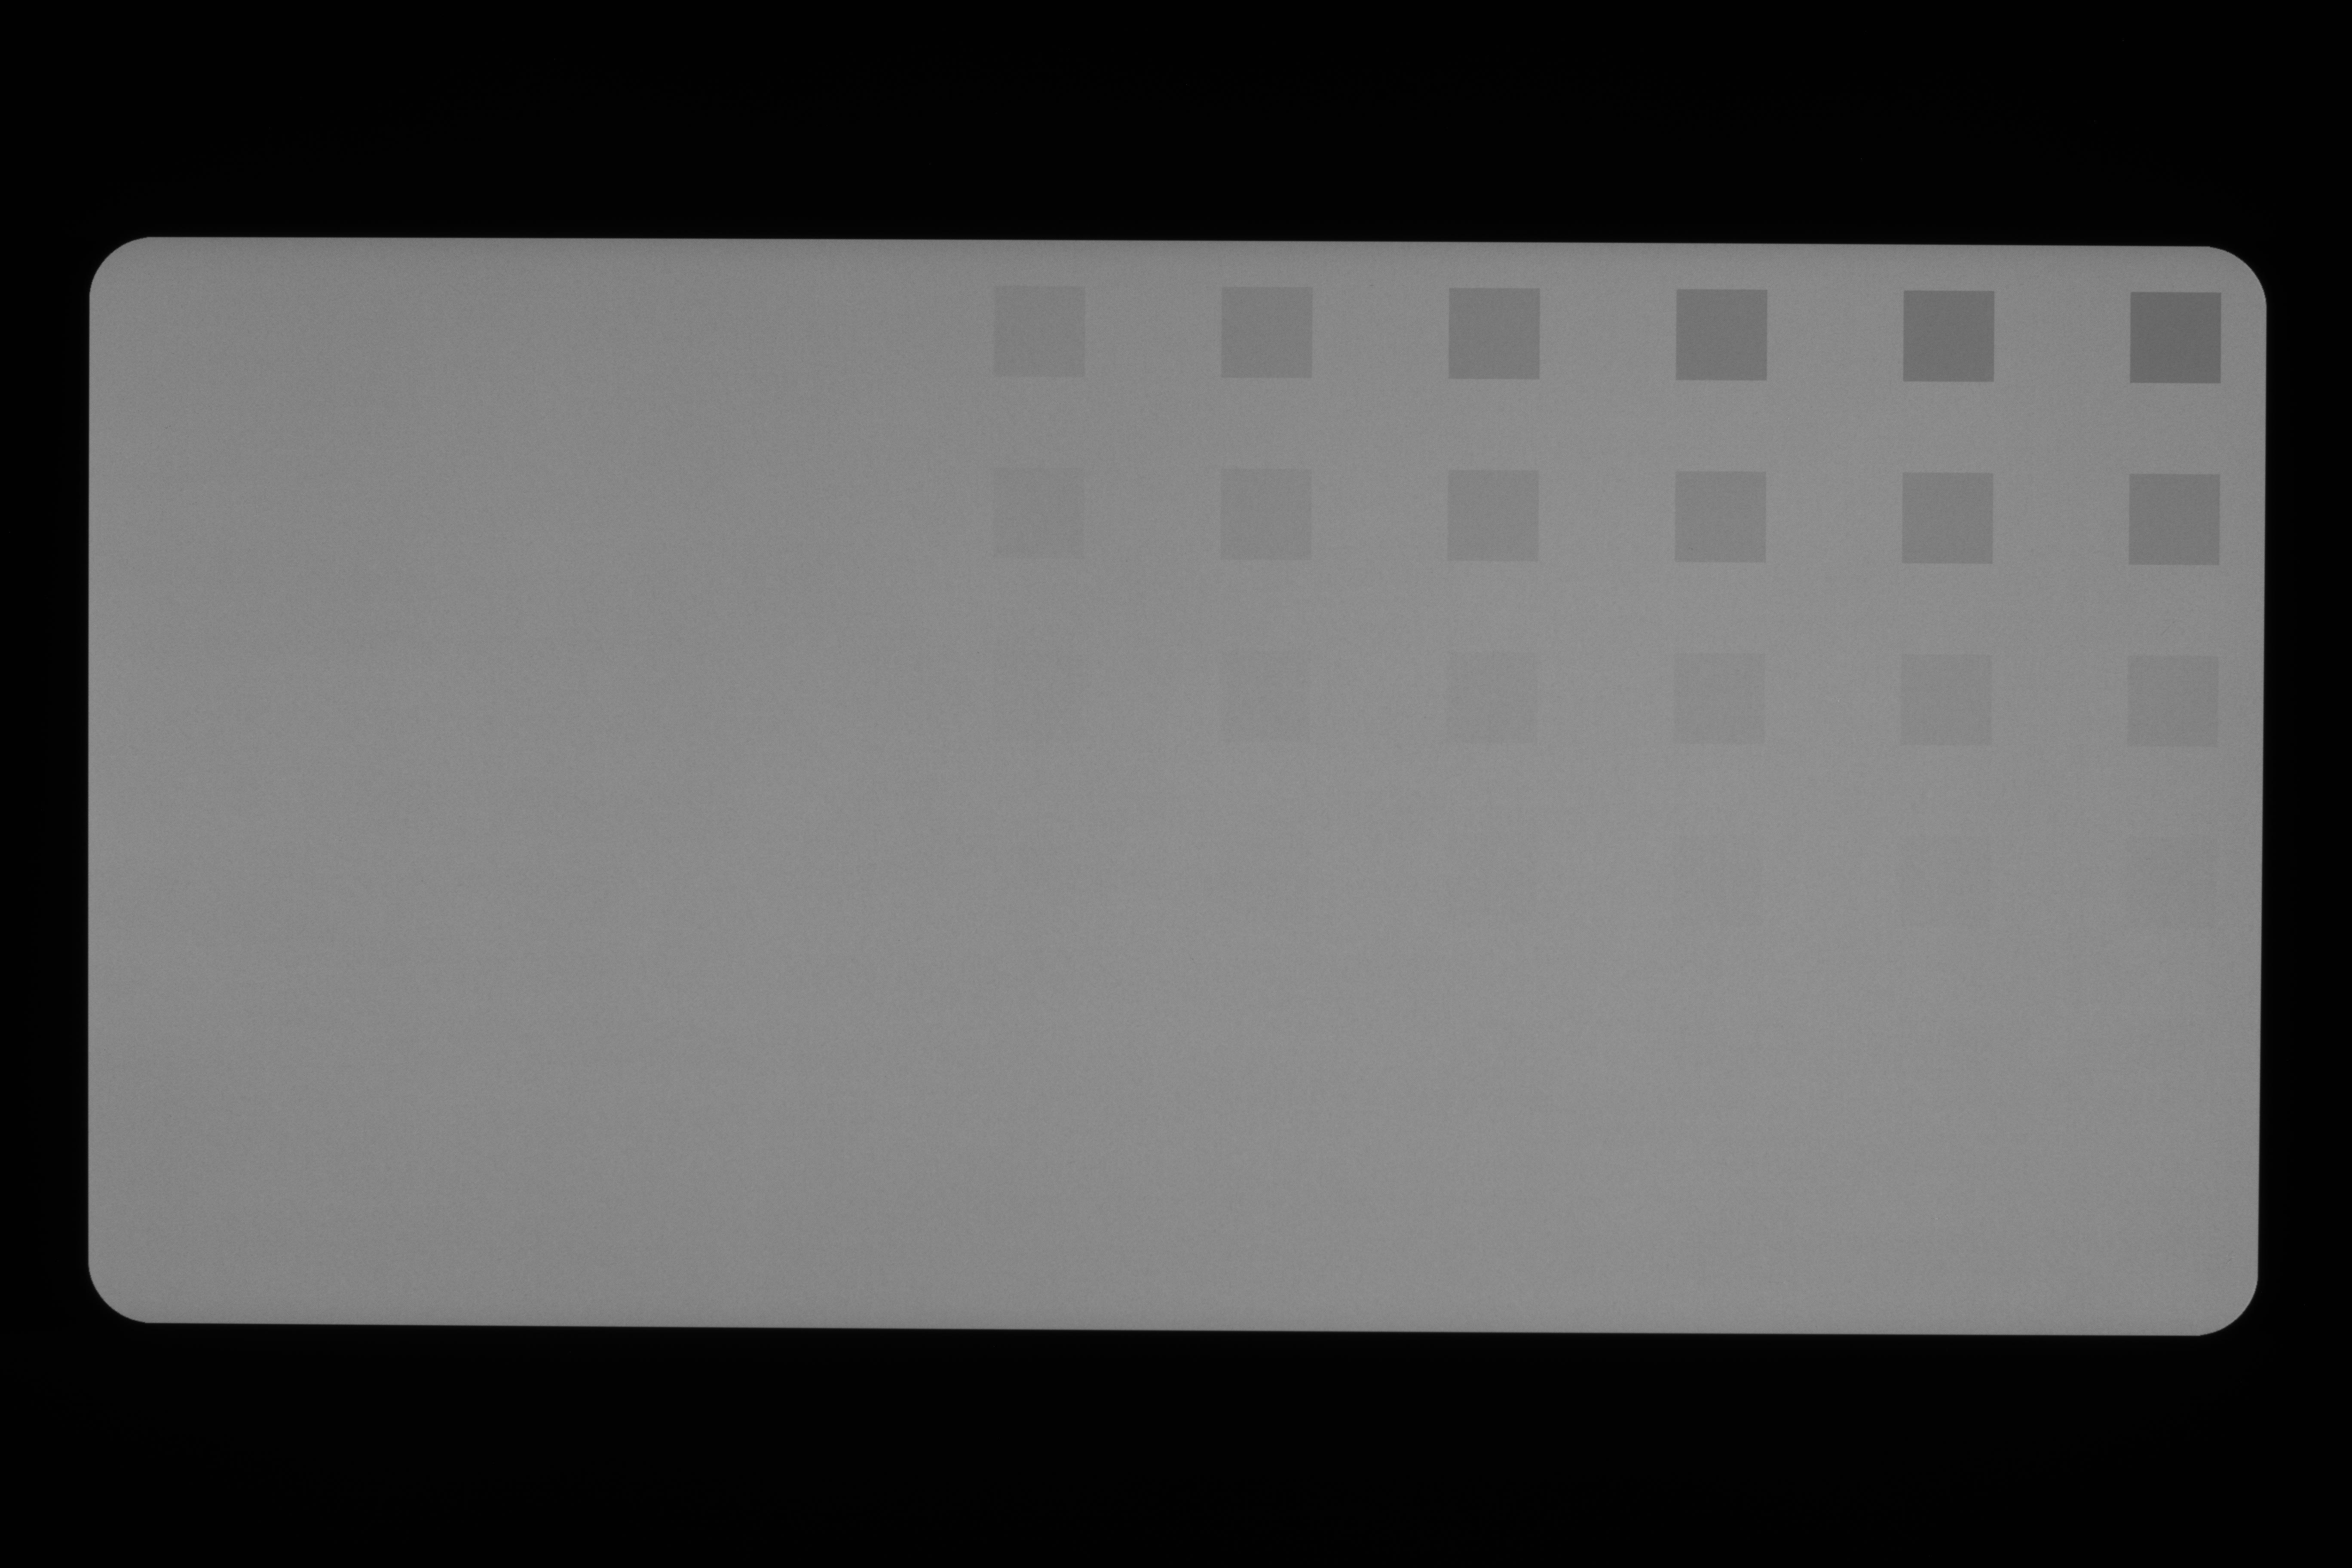
\includegraphics[width=0.6\textwidth]{uncomp.jpeg}
    \caption{An AMOLED display was aged and has OLED burn-in shown on display}
    \label{fig:1}
\end{figure}
\begin{figure}
    \centering
    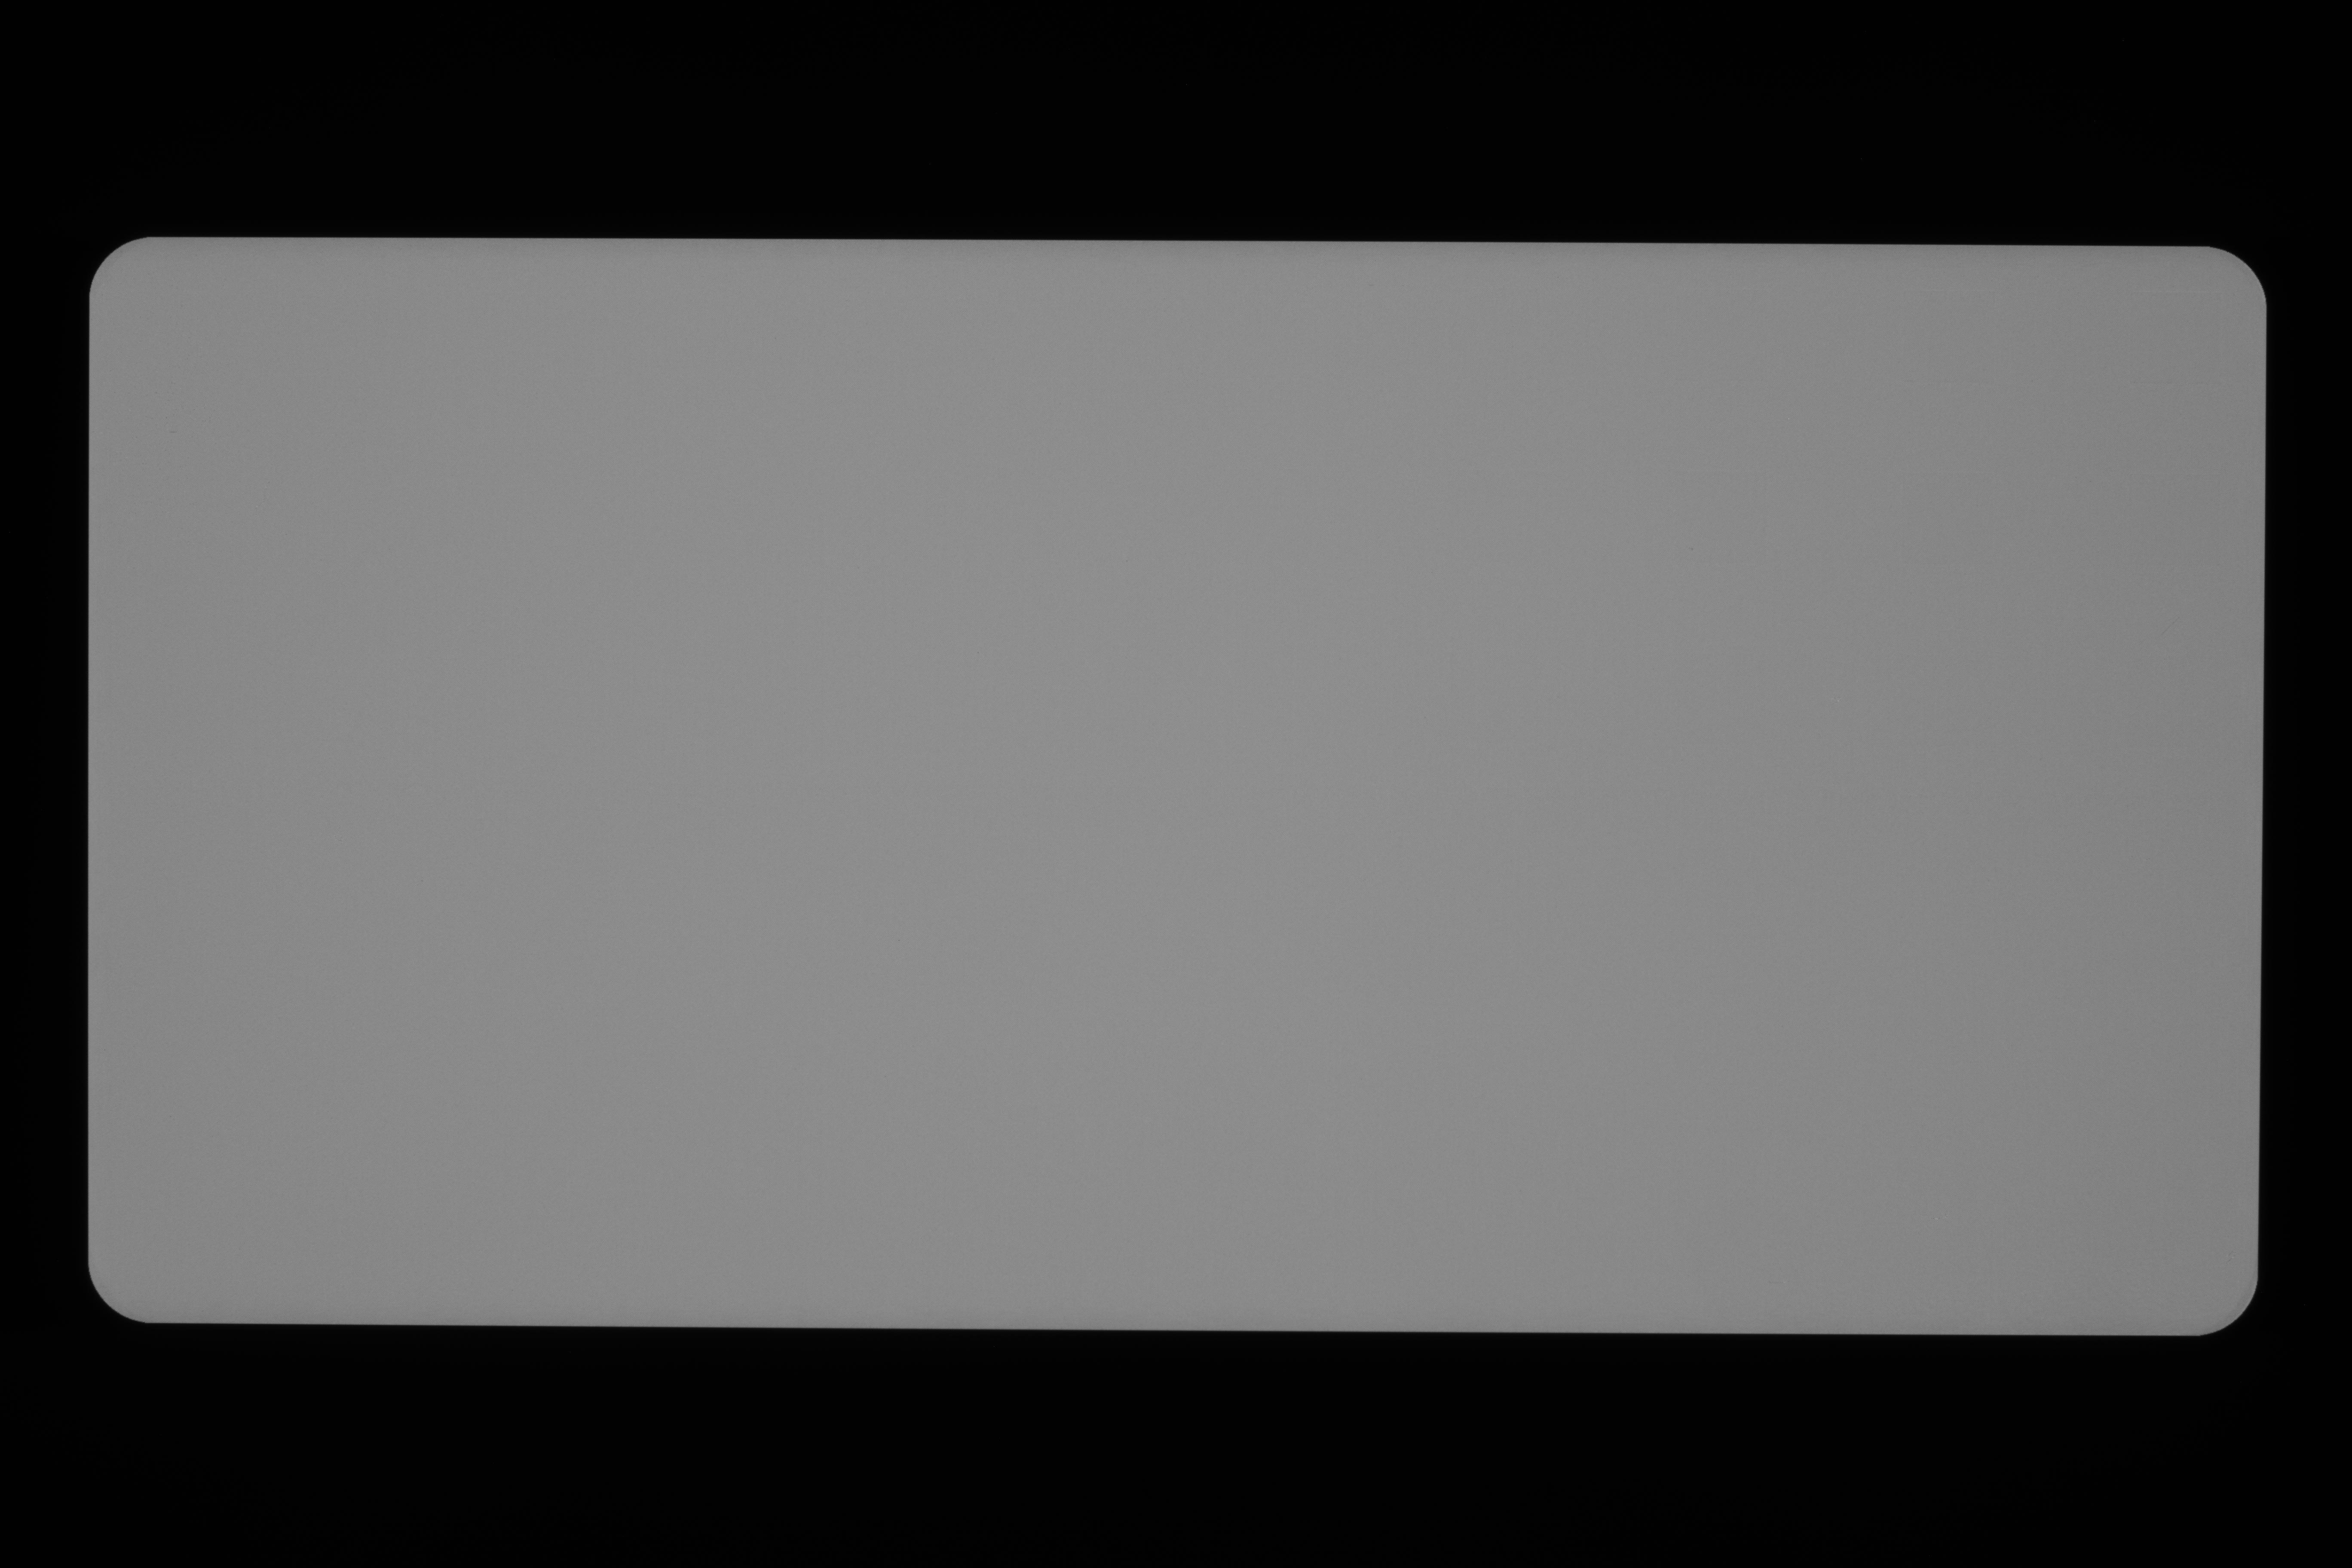
\includegraphics[width=0.6\textwidth]{comp.jpeg}
    \caption{With OLED ageing compensation,the same AMOLED display's burn-in is eliminated}
    \label{fig:2}
\end{figure}
%
%
\section{Literature review}
In order to archive the project, except the materials we learned from ECE657A course, we also referenced a numbers of papers in the fields of image processing, machine learning ,deep learning and AMOLED display technologies.

Accordingly, researches have been conducted into designing methods to evaluate luminance uniformity. For example, visual sensitivity characteristics are applied to a display image \cite{doi:10.1889,5985739,Kunihiko} and edge detection\cite{Chen_2007,ROVAMO19992387} and differential filtering \cite{doi:10.1002/sdtp.13087} are used to emphasize luminance non-uniformity. But those methods have unsatisfying performance under restricted conditions. However recent researches have opened up the possibility for using deep neural networks \cite{doi:10.1002/sdtp.13087} to evaluate luminance non-uniformity automatically, which enables optimization of feature quantity extraction.

Peter Barten’s research on the contrast sensitivity of human eye \cite{barten2003formula} provides a formula for contrast sensitivity which is helpful to improve accuracy of result by minimize the contrast sensitivity various of human eye. This can be done by implementing contrast sensitivity function to emphasis the difference between AMOLED display's normal areas and OLED aging areas.
Kazuki Tsutsukawa and his team at EIZO Corporation, developed an Evaluation system for Luminance Non-Uniformity Based on Deep Neural Networks\cite{doi:10.1002/sdtp.13087}. Their research paper shows that the possibility for using deep neural networks [4] to evaluate luminance non-uniformity automatically, which enables optimization of feature quantity extraction.
%
%
\section{Design Considerations}
Figure.\ref{system-diagram} shows a high level overall system diagram of our system. We will briefly discuss each part of the system in this section. We design the system under below considerations.
\clearpage
\begin{figure}[H]
    \centering
    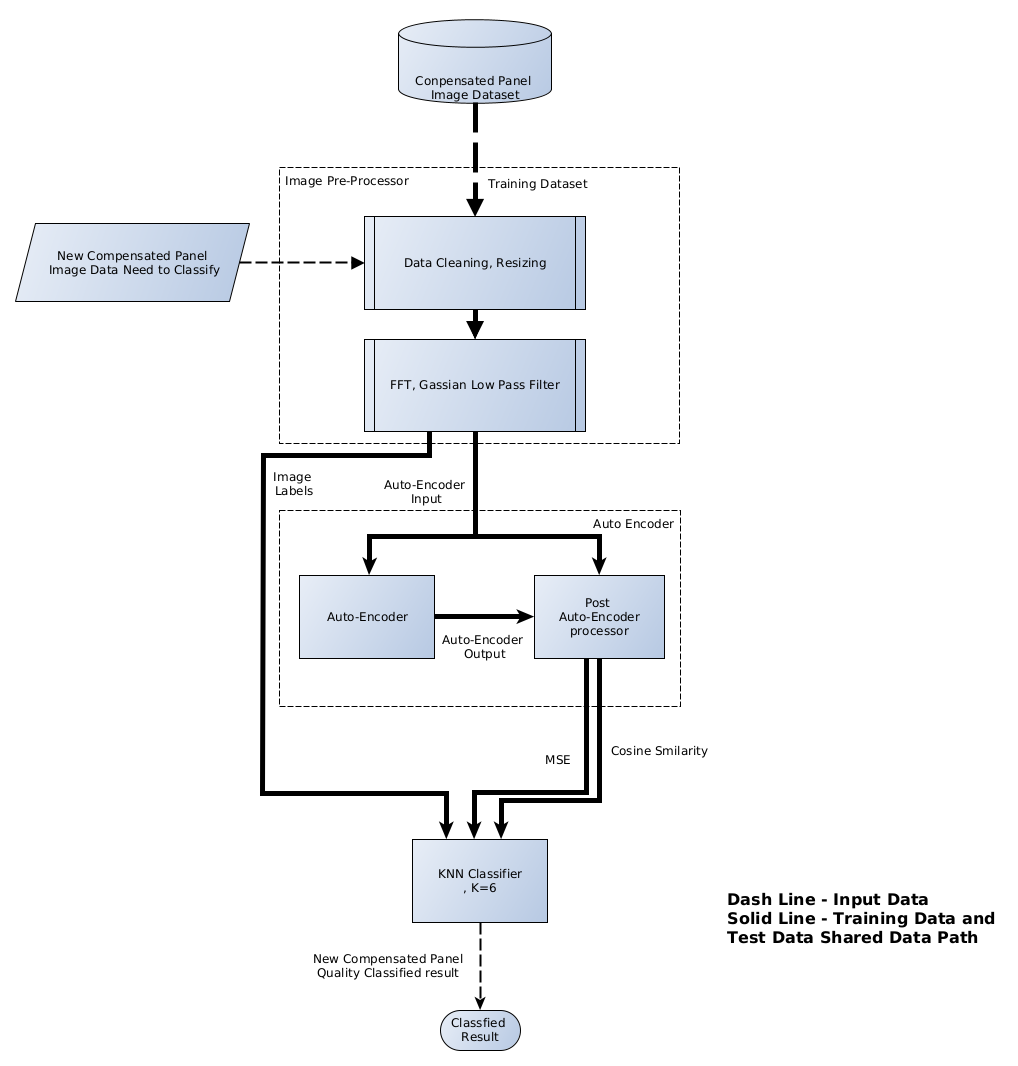
\includegraphics[width=0.9\textwidth]{system-diagram.png}
    \caption{System Design Diagram}
    \label{system-diagram}
\end{figure}

\subsection{System Input - Load Training Dataset}
The system shall take image files from a specified folder containing two sub-folders - “good” and “bad”. They stores the panel image files. Folder “good” contains panel images with good quality compensation; folder “bad” contains panel images with bad compensation quality. The image file shall be either jpeg or png format. The system will use these data folders as training datasets; the folder names “good” and “bad” will be used later in the project as the label.

\subsection{Data Pre-process}
After images were loaded, these images need to be pre-processed in order to fit into system to train system. We need to perform following steps as data pre-processing.
\begin{itemize}
    \item{Perform image data integrity check}
    \item{Data cleaning}
    \item{Resizing the image to meet speed requirement while keep data quality}
    \item{Run selected image filter to emphasis image’s the nonuniform area}
\end{itemize}

\subsection{Auto-encoder}
The auto-encoder takes pre-processed image data as input data fit into a convolutional auto-encoder, extracting the features via the encoder and reconstructing the image according to the features by the decoder. Parameters of the CAE are optimized to decrease differences between the inputs and outputs. Since the displays are all displaying a uniform gray picture, ideally, the reconstruction loss will be very low when inputting the image of a well-compensated display with few noises to be filtered.

Based on the input and output data of auto-encoder, two indicators, mean square error and cosine similarity, are calculated and used for evaluating the compensation quality.

\subsection{Find System Decision Boundary}
We use a set of pre-classified labelled panel image data taken in the past as dataset to train system. After the entire dataset went through auto-encoder, we shall get two-dimensional data arrays of MSE and Cosine similarity, fit this 2D data array with “good/bad” label information to a classifier, so that we shall be able to find good/bad compensation quality decision boundary.
\subsection{System Output}
Once the system and its classifier was trained, the system is ready to take testing set to detect whether the display panel had a good or bad quality compensation.
%
%
\section{System Implementation}
Based on the design considerations that we discussed in the previous section, we implemented the system with python. Here we will discuss more implementation details in this section.
\subsection{Image pre-processing}
Image pre-processor plays an important role in this system. The sample image loaded from the dataset should be formed into a specific format as the autoencoder requires and contribute to optimizing the autoencoder’s performance, including quality and speed. We have implemented several pre-processing functionalities mainly in two parts.

\subsubsection{Data cleaning and data resizing\\}
Figure. \ref{dataclean} shows AMOLED panel image before and after data cleaning process. The original image has a black edge taken by camera, which needs to be cut. And dark areas at four round corners need to be cleaned by filled with mean value.
\begin{figure}
    \centering
    \subfigure[Original panel Image]{
        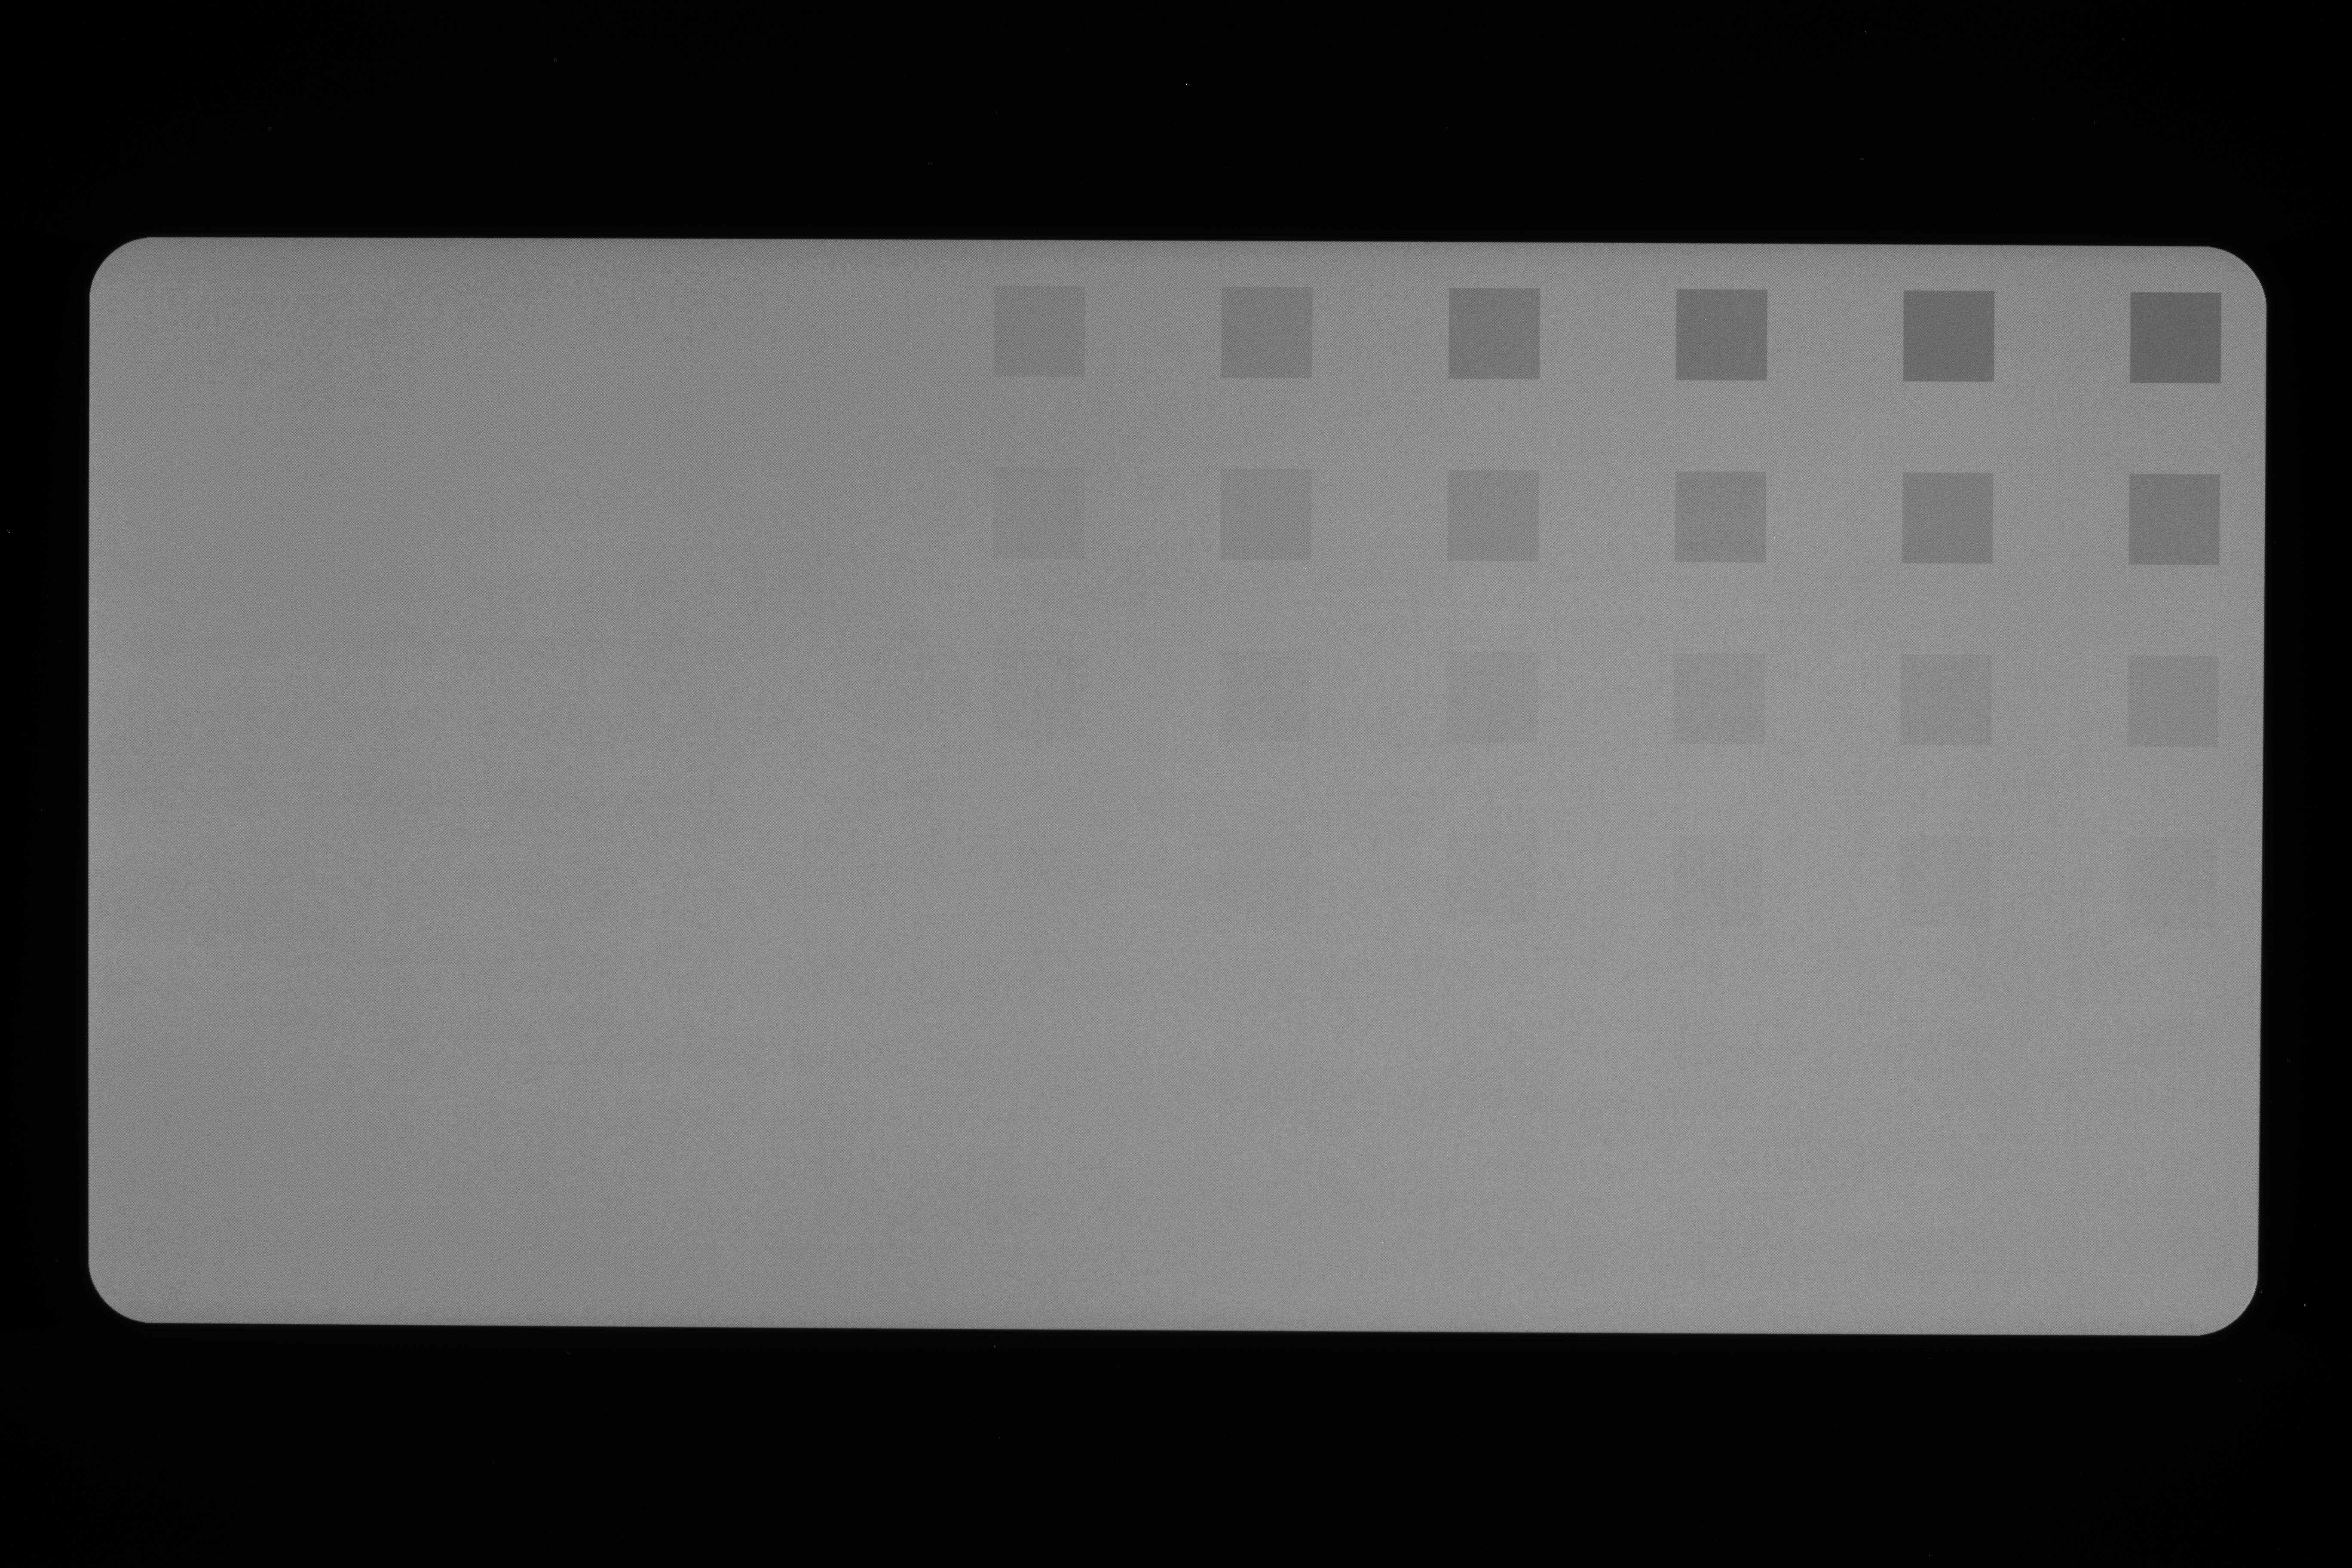
\includegraphics[width=0.4\textwidth]{Pixel2-uncomp-original.jpeg}}
   \subfigure[Panel Image After Data Cleaning]{
        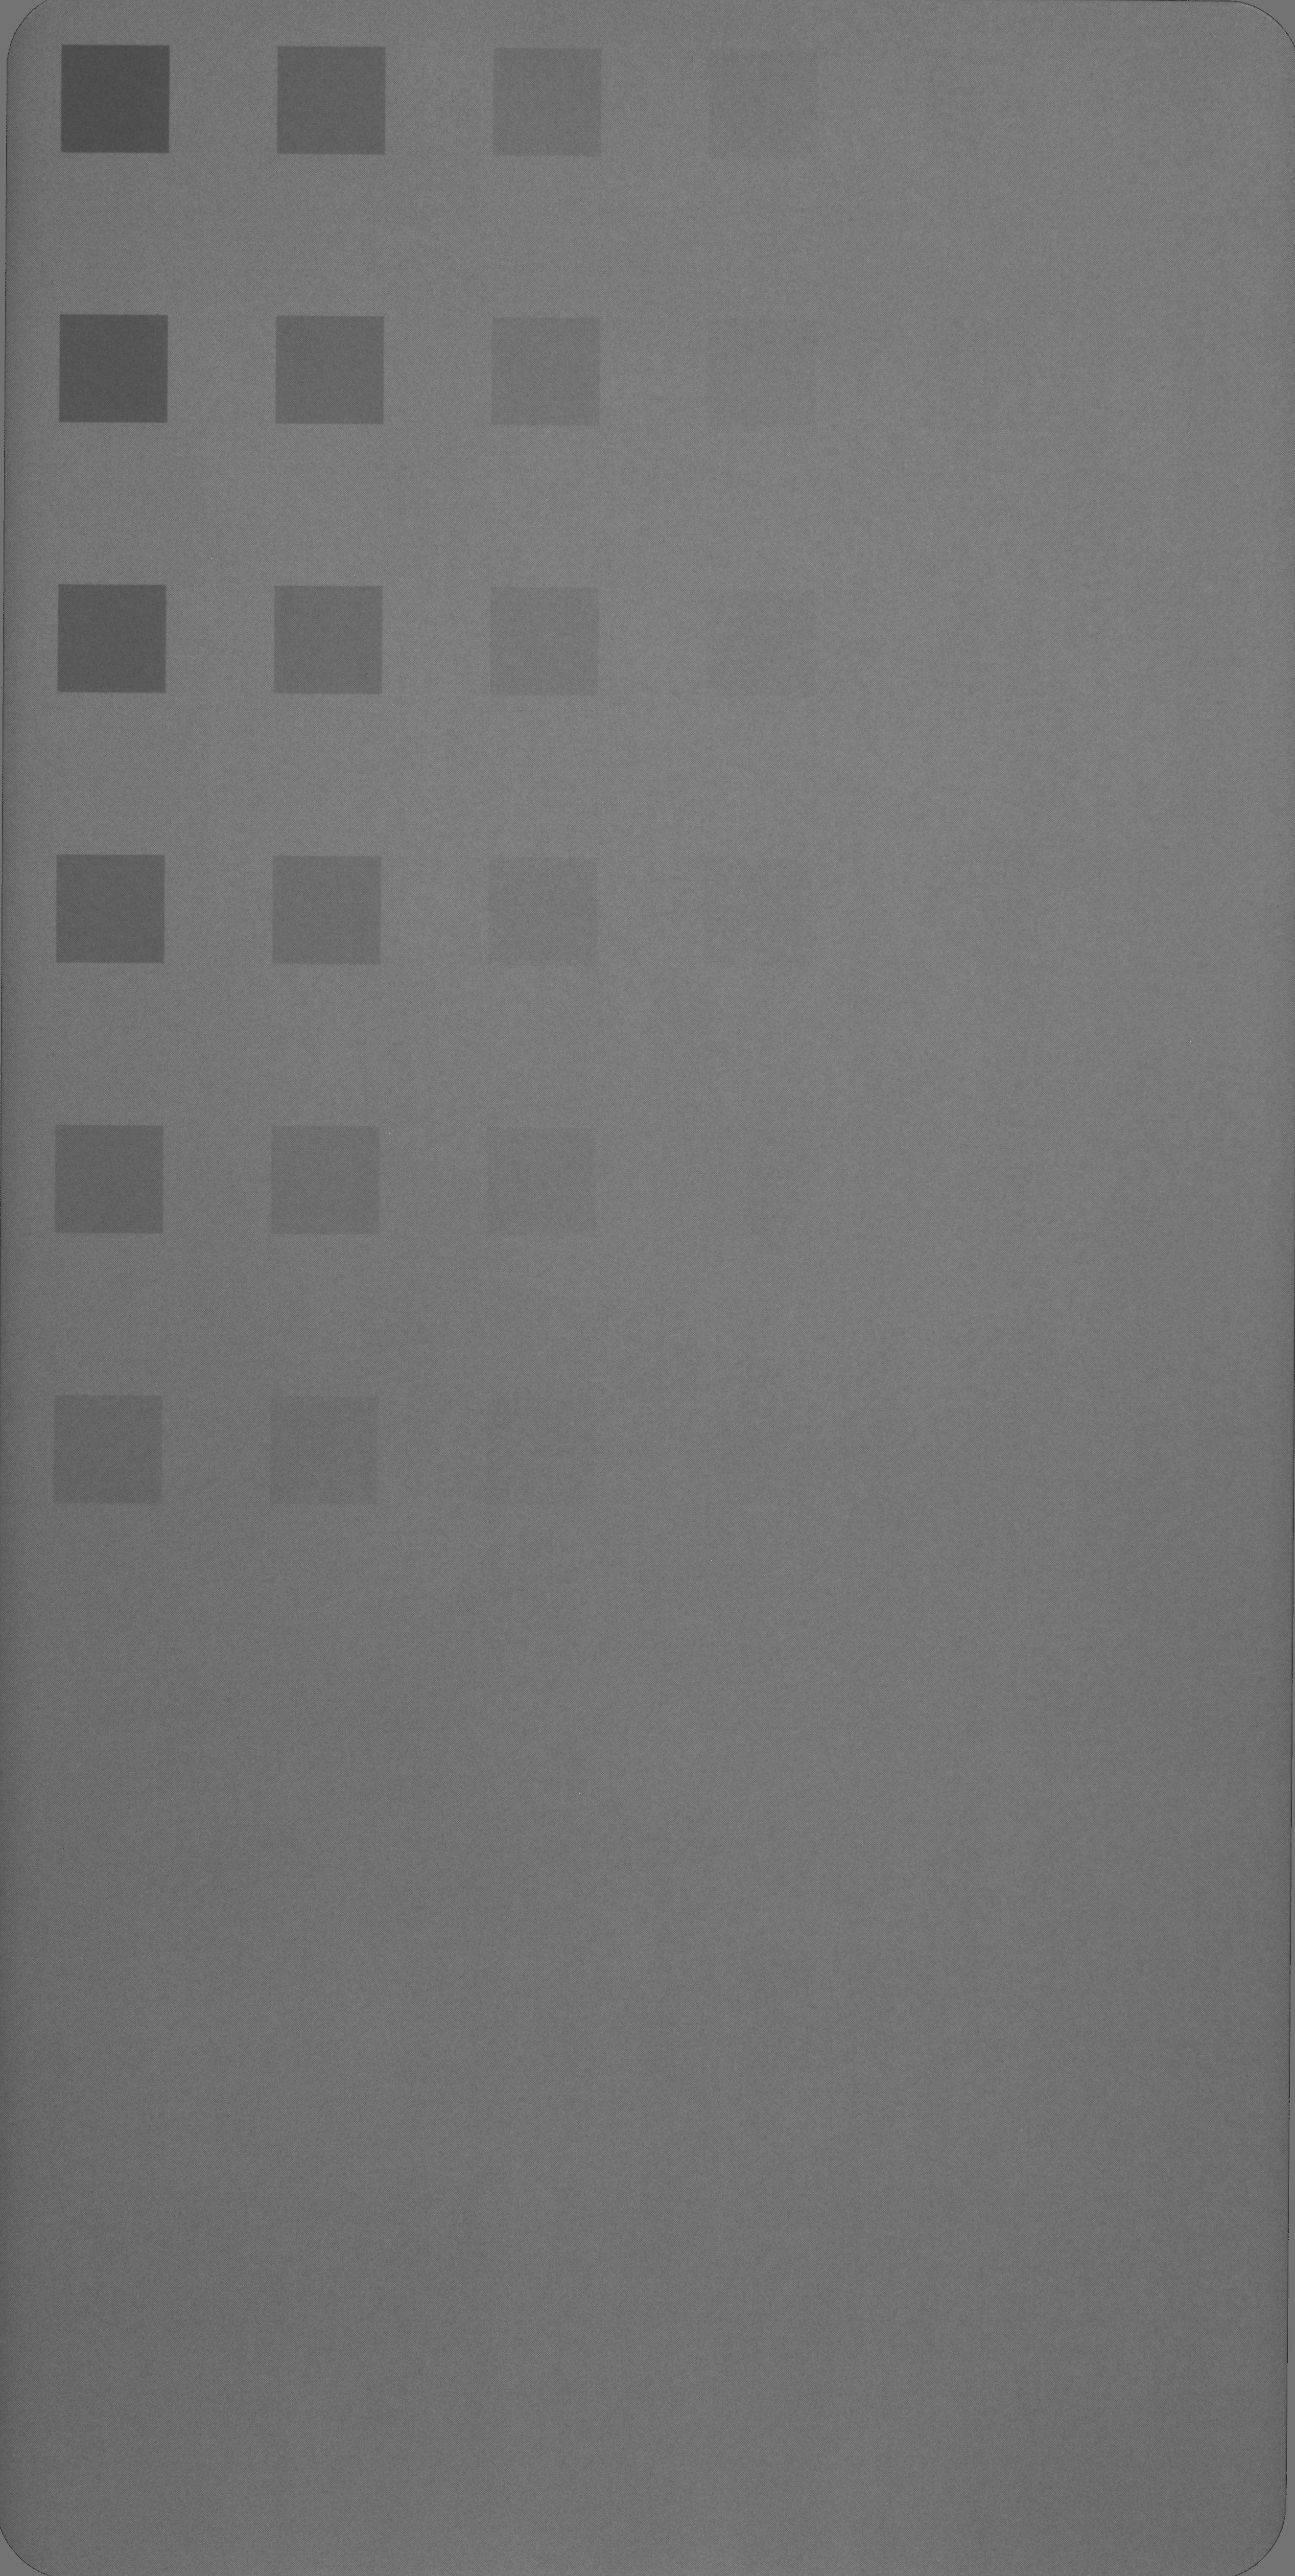
\includegraphics[width=0.2\textwidth]{Pixel2-Uncomp-g.jpeg}}
    \caption{Comparison of images before and after data cleaning}
    \label{dataclean}
\end{figure}

\subsubsection{Image data filtering\\}
As mentioned in our project proposal, we planned to implement a CSF (Contrast Sensitivity Function) to reduce the impact of the fact that vision sensitivity varies among different people. However, while we are working on implementation, we noticed that to be able to calculate the contrast sensitivity, we need four parameters, spatial frequency in cycle/degree, display luminance, surround luminance and Field of view in degree. We realized that we lacked the equipment to measure surround area luminance data during the panel measurement. As the trade-off, we decided to use the FFT-Gaussian-LowPass filter instead of using CSF to enhance the luminance difference between the nonuniform and uniform areas of AMOLED panels. The output from the FFT-Gaussian-LowPass filter is used as the auto-encoder’s input.

\begin{figure}
    \centering
    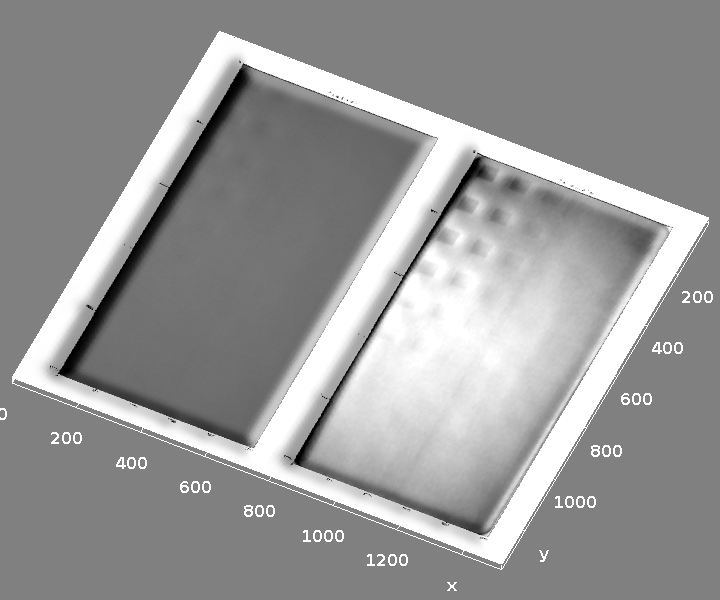
\includegraphics[width=0.8\textwidth]{Surface_Plot_of_3D_plot_resized_fft_lowpass.png}
    \caption{Image Data before and after FFT Gaussian Low Pass Filter}
    \label{3Dplot}
\end{figure}


Fig.\ref{3Dplot} shows that the pre-processed original image and the image after the FFT-Gaussian-Lowpass filter processed. The image was taken from a panel that had applied for OLED compensation on the panel. However, the compensation was not perfect, as we can still see slight burn-in on the panel. Comparing the left side of the plot with the right side of the plot, we can clearly see that after FFT-Gaussian-Lowpass filter processing, the luminance difference between the compensated area and normal areas was emphasized by the filter.

After the phase of image pre-processing, the pre-processed data will be passed to the next major module - the CNN based auto-encoder.
\subsection{CNN based Auto-encoder}
A convolutional auto-encoder (CAE) deep neural network was designed as the first step of classification, which takes pre-processed photos of the display as inputs and outputs the same size data to generate the indicates for evaluating compensation quality. Table. \ref{tab:cae} is the structure of the CAE. The encoder of CAE consists of 4 convolutional layers, 1 flatten layer and 1 fully-connected layer, which extracts the main features from the inputs into a vector with 1024 dimensions.  The decoder consists of 1 fully-connected layer, 1 reshape layer and 4 deconvolutional layers, which reconstruct the 1024-dimensional vector into an image with the same size as the input.
\begin{table}
    \centering
    \caption{Structure of the CAE}
    \label{tab:cae}
    \begin{tabular}{ccccc}
        \toprule
        Layer (type) & $\quad$ &  Output Shape & $\quad$ &  Param \#\\
        \midrule
        1st convolutional layer & \ & (None, 70, 54, 32) & \ &  320 \\
        2nd convolutional layer & \ &  (None, 34, 26, 64) & \ &  18496 \\
        3rd convolutional layer & \ &  (None, 16, 12, 128) & \ &  73856 \\
        4th convolutional layer & \ &  (None, 7, 5, 256)  & \ &  295168 \\
        Flatten layer & \ &  (None, 8960) & \ &  0 \\
        1st fully-connected layer & \ &  (None, 1024) & \ &  9176064 \\
        2nd fully-connected layer & \ &  (None, 8960) & \ & 9184000 \\
        Reshape & \  &  (None, 7, 5, 256) & \ &  0 \\
        1st deconvolutional layer & \  & (None, 16, 12, 128) & \ &  524416\\
        2nd deconvolutional layer & \ &  (None, 34, 26, 64) & \ &  131136  \\
        3rd deconvolutional layer & \ &  (None, 70, 54, 32) & \  &  32800 \\
        4th deconvolutional layer & \ &  (None, 141, 110, 1) & \ &  385 \\
        \bottomrule
    \end{tabular}
\end{table}

\subsection{Choose Classifier and Decision Boundary}

\begin{figure}[H]
    \centering
    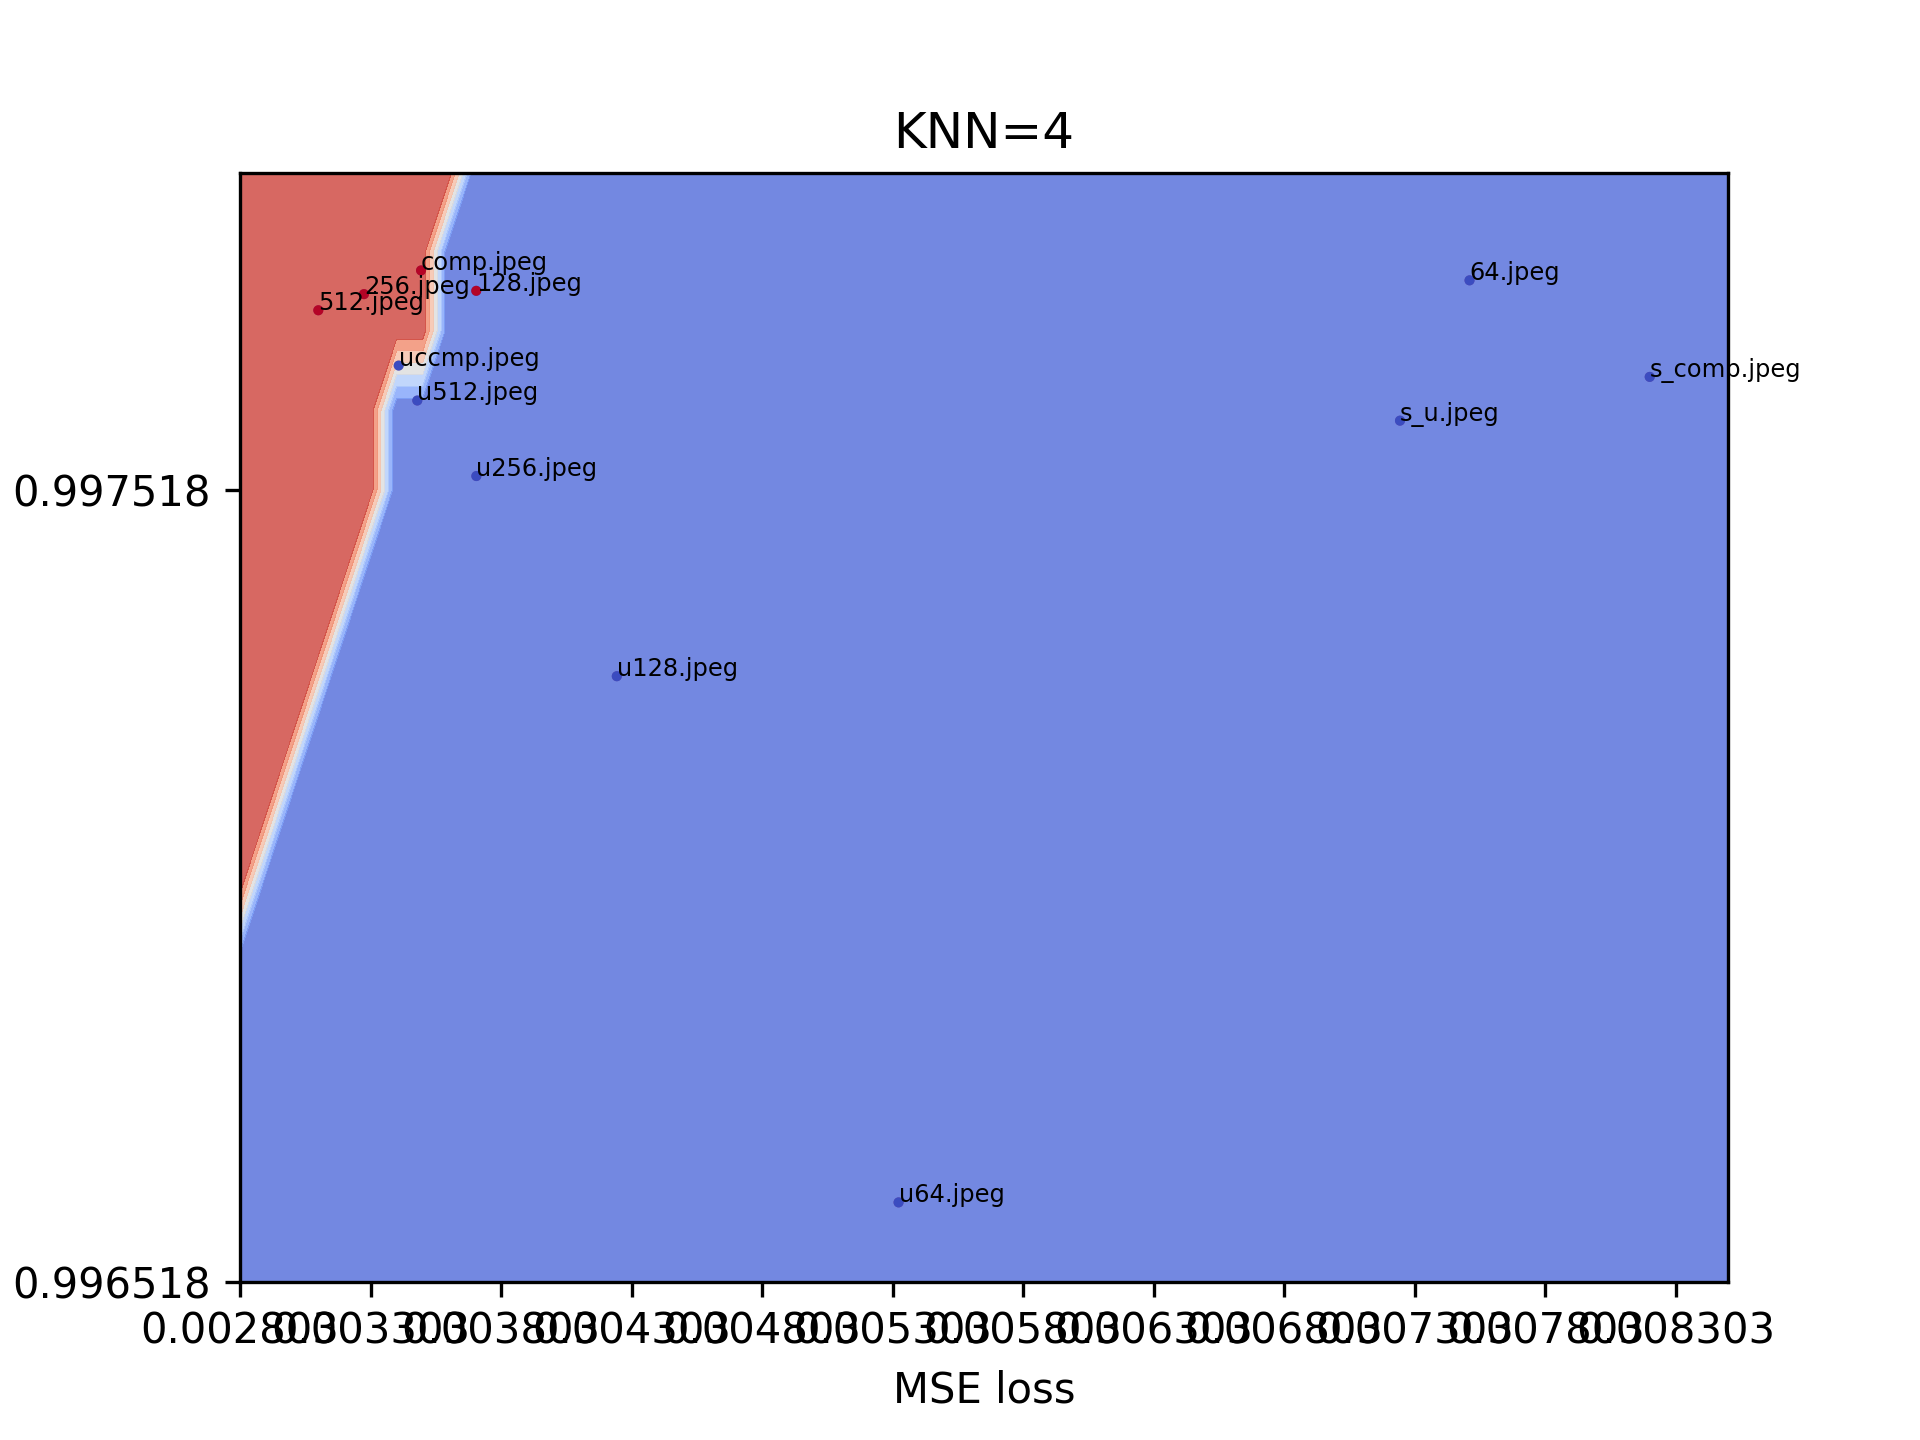
\includegraphics[width=0.9\textwidth]{decision-boundary.png}
    \caption{Decision Boundary}
    \label{decisionBound}
\end{figure}

From auto-encoder, we get two sets of compensation quality evaluation indicators. MSE and Cosine Similarity. The next step is use these indicators and image sample label to train classifier, Classifier is trained with training dataset, after training the system is ready for the AMOLED ageing compensation quality classification.

Due to the limited samples, it gave us some difficulty to choose a classifier with better performance, and clear decision boundary. We took some time to work on choosing suitable classifier for this project. Based on current image samples, finally we chose KNN as classifier with K equal to 6. Figure. \ref{decisionBound} shows comparison of decision boundary based on training samples.

As we can see, the KNN algorithm shows clearest boundary than others, some of the algorithm even couldn't find a decision boundary under the same condition as KNN has. The decision boundary plot based on two performance indicators. The Y axis is Cosine similarity, and X Axis is Mean Square Error, any image sample fall into the Left-Upper corner of the plot indicates the high compensation quality, on the other side indicates bad compensation quality.

In the future as we could get more image samples, we would redo the evaluation for the classifier selection, and then we could have more accurate decision boundary based on larger dataset as compensation quality selection base.

\section{System Validation}
Once decided to use KNN classifier with K equal to 6,  we validated system with following procedure.
\subsubsection{Testing and Result Accuracy}
We use total 87 panel images as trainig dataset, and take another 22 panel images as test dataset. These panel images were pre-classified and labeled manually in the previous work. There are 8 sample images labeled as "Good" and 14 sample images labeled as "Bad" within test dataset. Both training dataset and test dataset ran through the pre-processing and auto-encoder, then we got MSE and Cosine similarity sets for training datseta and test dataset. Fit training dataset MSE/cosine similarity to KNN classifier first, then fit test dataset's MSE/cosine similarity to KNN classifier to get predicted result.
Finally we got confusion matrix as Table.\ref{tab:cm}, based on confusion matrix we calculated classifier accuracy was 95.5\%, and classifier precision was 96.7\%\\
\begin{table}
    \centering
    \caption{Classifier Confusion Matrix}
    \label{tab:cm}
    \begin{tabular}{cc}
         & Actual \\
        Predicted & $\begin{bmatrix} 14 & & 0 \\ 1 & & 7\\ \end{bmatrix}$\\
    \end{tabular}
\end{table}
\subsubsection{System performance}
We ran the test on a PC with Intel-i7 8Cores CPU, Intel HD-Graphics630 GPU and 15.5GB RAM. For 109 sample images ran through all processes (pre-processing, auto-encoder, classification) took 108.7 seconds. As average it about 1 second per sample. Considering the decision boundary has been decided by training dataset. This running time (1 second) will be every new test sample's running time. Compare with manually detect compensation image quality by human vision, this result is pretty impressive.

\section{Discussion}
How to evaluate the quality of compensation of AMOLED display panel in an accurate and fast way, is technical challenge. For comparison, we also ran a experiment with a pure classification process with SVM with linear and RBF kernel. Both svm kernels brought us lower accuracy about 57.1\% and 65.2\%. This shows that difficulty of feature extracting and evaluate the luminance difference accurately between good and bad compensation. Because of that, using a pure classic classifier like SVM to evaluate panel image luminance uniformity couldn't bring us accurate result.\\
Our approach is focus on emphasis the luminance differences by using FFT-Gaussian-lowpass filter, and furthermore, using a convolution neural network based auto-encoder, at end calculate two indicators MSE and cosine similarity, and use them to identify the image quality class to give us better accuracy for about 95.5\% .
\section{Conclusion and Future work}
\subsection{Conclution}
In this project we were able to build a rapid AMOLED aging compensation evaluation system based on the knowledge that we learned in course ECE657A. We designed and implemented the system which is consist of an image pre-processor, a Convolution Auto Encoder, and a Classifier. The overall performance is about 1 second of image processing time and 95.5\% of accuracy, this result is impressive to compare with human vision based manual classification process.
\subsection{Future work}
As the consideration of future work, here are few points we would improve in the future.
\subsubsection{Retrain the system with larger sample dataset}
Larger sample set always helps to improve system accuracy, especially help for finding more accurate decision boundary. Re-select suitable classifier if needed.
\subsubsection{To improve classification}
Now we can classify AMOLED aging compensation is Good or Bad compensation. However, it will be great to classify bad compensation as Under-compensated or Over-compensated. That is important function for an automated AMOLED panel calibration system. It could get feedback from evaluation system to know whether the panel is under-compensated or over-compensated to adjust compensation accuracy.
%
% ---- Bibliography ----
%
% BibTeX users should specify bibliography style 'splncs04'.
% References will then be sorted and formatted in the correct style.
%
% \bibliographystyle{splncs04}
% \bibliography{mybibliography}
%
\bibliography{proposal}
\bibliographystyle{splncs04}
\end{document}
